\label{sec:bts:revenue:expenses}

\begin{figure*}[!htp]
 \centering
 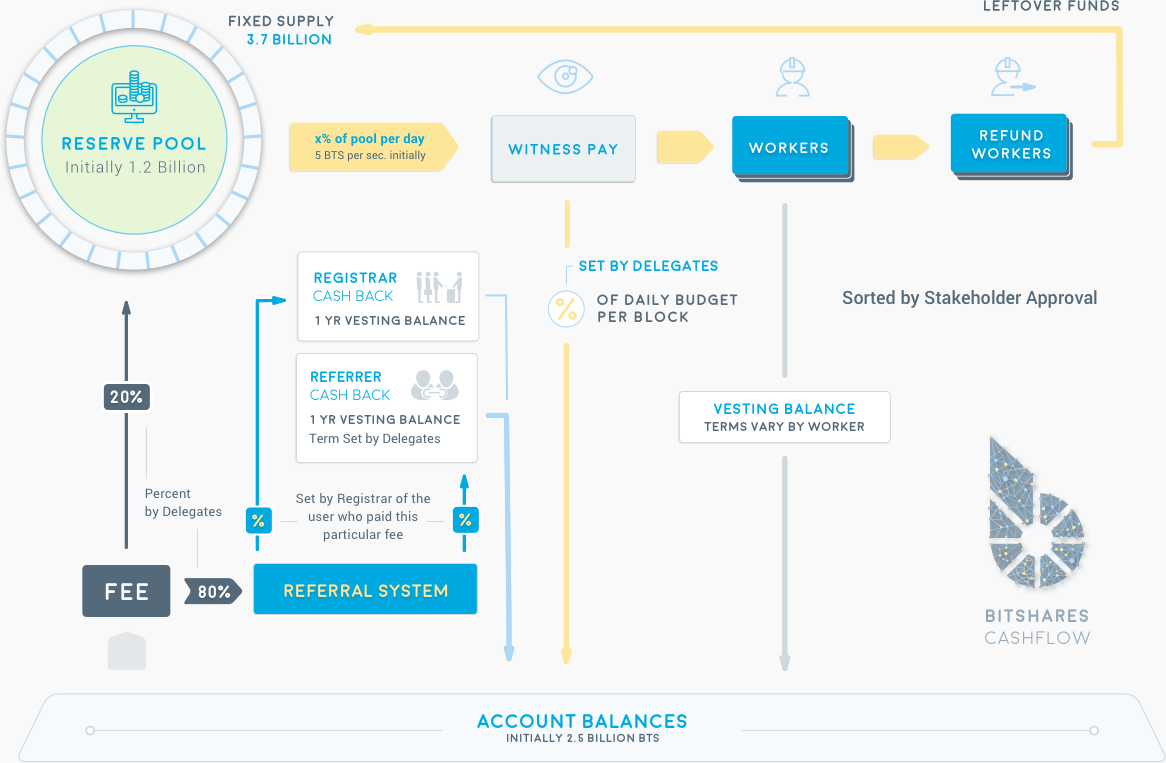
\includegraphics[width=.8\linewidth]{figures/cashflow.png}
 \caption{Cash flow of BitShares 2.0}
 \label{fig:cashflow}
\end{figure*}

%% Revenue
Revenue streams are essentially caused by fees that have to be payed when using
the DACs products, such as market pegged assets, user-issued assets, or the
decentralized exchange~\cite{bts:financial}. These fees are variable, can be
changed by shareholder approval and include
\begin{inparaenum}[(a)]
 \item transfers,
 \item order operations,
 \item account operations,
 \item asset operations,
 \item witness creations
 \item proposal operations
 \item withdraw permission operations
 \item committee member operations,
 \item worker creation,
\end{inparaenum}
and more.

%% Costs
In contrast to bitcoin, where newly created coins in each block are distributed
solely among countless miners that immensely overpay for the network
security~\cite{ltb:dac}, the BitShares ecosystem achieves a better security at
lower costs by means of an adjustable number of approved and trusted witnesses
in DPOS. Additionally, the BitShares ecosystem has the capability to pay for
its own development through budget items. Both, the payment for witnesses, as
well as the budget items are required to be approved by the shareholders.

As an example, an entrepreneur may approach the shareholders and offer to
launch a business in the BitShares space that would greatly benefit the
ecosystem. If he succeeds and convinces the shareholders to vote for and not
against his plan, he could get an initial funding by the DAC.

Another use-case would be the improvement of the blockchain's protocol. A
developer could propose a change or extension of the existing software
implementation and be payed by the DAC to do so (after shareholder approval).
Hence, as long as the average shareholders acts rational, the BitShares
blockchain can be seen as a self-funded but profitable business
